\documentclass[UTF8]{beamer}
\usepackage[space,hyperref]{ctex}
\usetheme{Warsaw}  %主题
\setbeamertemplate{caption}[numbered]
\setbeamertemplate{navigation symbols}{}%去除导航符号
\author{向涛}
\title{有限差分求解抛物方程}
\institute{数学与计算科学学院}
\titlegraphic{
\includegraphics[width=0.35\textwidth]{logo.jpeg}}
\begin{document}
\frame{\titlepage} % 标题页贞

\begin{frame}[c]\frametitle{itemize}

\begin{enumerate}
\item 引言
\item 抛物方程模型
\item 方程求解思路
\item 空间离散和时间离散
\item 线性方程的求解
\item 求解结果
\item 结果分析
\end{enumerate}

\end{frame}

\begin{frame}[t]\frametitle{引言}

微积分方程这门学科产生于十八世纪,欧拉在他的著作中最早提出了弦振动的二阶方程,随后不久,法国数学家达朗贝尔也在他的著作《论动力学》中提出了特殊的偏微分方程。不过这些著作当时没有引起多大注意。
1746年,达朗贝尔在他的论文《张紧的弦振动时形成的曲线的研究》中,提议证明无穷多种和正弦曲线不同的曲线是振动的模式。这样就由对弦振动的研究开创了偏微分方程这门学科。
和欧拉同时代的瑞士数学家丹尼尔·贝努利也研究了数学物理方面的问题,提出了解弹性系振动问题的一般方法,对偏微分方程的发展起了比较大的影响。拉格朗日也讨论了一阶偏微分方程,丰富了这门学科的内容。
偏微分方程得到迅速发展是在十九世纪,那时候,数学物理问题的研究繁荣起来了,许多数学家都对数学物理问题的解决做出了贡献。
这里应该提一提法国数学家傅立叶,他年轻的时候就是一个出色的数学学者。在从事热流动的研究中,写出了《热的解析理论》,在文章中他提出了三维空间的热方程,也就是一种偏微分方程。他的研究对偏微分方程的发展的影响是很大的。

\end{frame}

\begin{frame}[t]\frametitle{抛物方程模型}

一般来讲偏微分方程分类有三种,分别是椭圆型,抛物型,双曲型;本次实验报告主要讨论的是抛物型的偏微分方程,抛物型的偏微分方程中最经典的就是热传导方程,具体研究的方程模型如下:

\begin{equation}
\left \{
\begin{aligned}
& \dfrac{\partial u}{\partial t}-k\dfrac{\partial^2 u}{\partial x^2}=0 \\
& u(0,t)=0,~~u(1,t)=0,~~t\in [0,0.1] \\
& u(x,0) = e^{-\dfrac{(x-0.25)^2}{0.01}}+0.1*sin(20\pi x), x\in (0,1)
\end{aligned}
\right.
\end{equation}

物理意义:该方程中$u$表示与空间x(此处仅考虑一维)和时间t的取值有关,即用$u(x_j,t_k)$表示在空间位于$x_j$处,时间为$t_k$时候的温度,系数$k$的取值与材料的密度,热传导系数及比热熔有关,此处为了计算方便,假设$k=1$.其余的是边界条件,有了边界条件才能够利用计算机进行数值计算

\end{frame}

\begin{frame}[t]\frametitle{方程求解思路}

\begin{enumerate}
\item 选择合适的差分格式

有限差分求解一维抛物方程时常用的差分格式有三种,分别是向前差分,向后差分,Grank-Nicolson格式,其中向前差分格式是条件稳定,其余两种都是无条件稳定的.Grank-Nicolson格式的精度是最高的,但代价是它的时间复杂度要比向后差分格式大(多了个矩阵和向量相乘);本次选择使用向后差分格式求解较为稳妥.

\item 将抛物方程转换成求解线性方程组

通过上一步将微分方程转换成了差分方程,一个点对应一个差分方程,那么通过有限差分的剖分会形成很多个点,这样就会有多个差分方程,最终形成一个差分方程组,写成矩阵和向量相乘的形式就可以理解成常规的线性方程组.对于抛物方程而言,我们一般是用一个线性方程组求解一个时间层的温度分布后然后通过循环就可以求解其他时间层的温度分布,逐次往上求解,这样整个抛物方程就求解完了.

\end{enumerate}

\end{frame}

\begin{frame}[t]\frametitle{空间离散和时间离散}

向后差分格式是一种隐式的求解格式,需要求解线性方程组.在求解方程前我们需要对求解的区域进行网格剖分,取空间步长和时间步长分别为$h=\dfrac{I}{N},\tau= \dfrac{T}{M}$,对空间变量$x$所属的区间$[0,I]$和时间变量$t$所属的区间$[0,T]$做如下均匀剖分:

\begin{equation}
0=x_0<x_1<\cdots<x_N=I,~0=t_0<t_1<\cdots<t_M=T
\end{equation}

其中$x_i = ih,t_k=K\tau~~i=0,1,\cdots,N~~K=0,1,\cdots,M$.

用两族平行直线$x=x_j(0,1,\cdots,N)$和$t=t_k(k=0,1,\cdots,M)$将求解区域分割为网格形式,对网格的节点我们用记号表示为:

\begin{equation*}
\left \{
\begin{aligned}
& \overline{G}=G_h \cup \Gamma_h=\{ (x_j,t_k):0\leq j\leq N;0\leq k \leq M \} \\
& G_h = \{ (x_j,t_k):0<j<N;0<k\leq M \} \\
& \Gamma_h=\{ (x_j,t_k):j=0,N;k=1,\cdots,M \} \cup \{  (x_j,t_0):j=0,\cdots,N \}
\end{aligned}
\right.
\end{equation*}

\end{frame}

\begin{frame}[t]\frametitle{空间离散和时间离散}

向后差分格式所用的模板点为:

\begin{center}
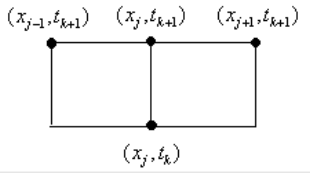
\includegraphics[scale=0.4]{1.png}
\end{center}

对于任意一点$(x_j,t_{k+1})$处的微分方程$\dfrac{\partial u}{\partial t} = \dfrac{\partial^2 u}{\partial x^2}$,我们用差商代替微分便有

\begin{equation}
\dfrac{u_j^{k+1}-u_j^k}{\tau} = \dfrac{u_{j+1}^{k+1}-2u_j^{k+1}+u_{j-1}^{k+1}}{h^2}
\end{equation}

$(3)$就是向后差分格式.

\end{frame}

\begin{frame}[t]\frametitle{空间离散和时间离散}

对$(3)$式两边同时乘以$\tau$,然后可以化简成如下的形式

\begin{equation}
-ru_{j-1}^{k+1}+(1+2r)u_j^{k+1}-ru_{j+1}^{k+1}=u_j^k
\end{equation}

其中$r=\dfrac{\tau}{h^2}$称为网格比,将$(4)$式写成矩阵形式就是

\begin{equation}
AU^{k+1}=U^k
\end{equation}

其中$A$的形式为

\[
\mathbf{A}=\left [ 
\begin{array}{ccccc}
1+2r & -r &  &  & \\
-r & 1+2r & -r &  & \\
   & \ddots & \ddots & \ddots & \\
 &  & -r & 1+2r & -r \\
 &  &  &-r  &1+2r 
\end{array}
 \right]
\]

\end{frame}

\begin{frame}[t]\frametitle{线性方程的求解}

现在我们已经将抛物方程$(1)$转化成求解线性方程组$(5)$式,对于编程求解而言,此时问题已经变得非常的简单了,比如对于$matlab~python$等语言,他们内部已经提供了求解线性方程组的命令,因此可以直接求解,但是他们的计算方式是理论上的常规算法,即矩阵和矩阵相乘会用到三次循环,那么矩阵若是$n$维的话,时间复杂度就是$O(n^3)$,矩阵乘向量也会达到$O(n^2)$.此外$(5)$还涉及到矩阵求逆,时间复杂度就会变的非常的高了,对于我们规模较小而言还可能会实现,规模一旦变大,将是一个不可能的现实.因此我的做法是用迭代方法代替矩阵求逆,此外迭代方法的内部也会用到矩阵和向量相乘的情况,我采用的是用压缩矩阵法$(CSR)$进行计算,这无疑会节省很多的运行时间(经我的电脑测试,对于二维的抛物方程求解而言,当$x~y$轴的划分均为60个内部节点,时间划分为400层的时候,利用内部命令直接求解就运行了296秒,而利用jacabi迭代并采用CSR的方法只运行了6秒,相差了50倍)

\end{frame}

\begin{frame}[t]\frametitle{线性方程的求解}

一般来说线性方程组的迭代法有很多,比如Jacobi,Gauss-seidel等,这里我采用的是Jacobi迭代方法求解线性方程组,具体的思路就是考虑分裂A=D-L-U,其中D是A的对角线部分,-L和-U分别为A的严格下三角和严格上三角部分,即可得Jacobi迭代方法:
\begin{equation}
x^{(k+1)} = D^{-1}(L+U)x_{(k)}+D^{-1}b,~k=1,2,\cdots,n.
\end{equation}
对应迭代矩阵为
\begin{equation}
G_{J}=(D)^{-1}(L+U).
\end{equation}

即可得到分量形式
\begin{equation}
x^{(k+1)}_i = \frac{1}{a_{ii}}\left(b_i-\sum^{n}_{j=1,j\neq i}a_{ij}x^{(k)}_j ,i=1,2,\cdots,n. \right)
\end{equation}

然后利用计算机进行编程求解

\end{frame}

\begin{frame}[t]\frametitle{线性方程的求解}

这里为什么要采用CSR方式呢?因为观察到$(5)$的矩阵$A$的零元素很多,只有对角和次对角才有非零元素,而CSR方式会将零元素忽略,所以当矩阵和向量相乘时会节约很多的时间,下面是一个CSR例子

\[
\mathbf{B}=\left [ 
\begin{array}{ccc}
1 & 0 & 2 \\ 
0 & 4 & 3 \\ 
0 & 5 & 6 \\ 
\end{array}
 \right]
\]

\begin{equation*}
\begin{aligned}
data = [1,2,4,3,5,6] \\
indices = [0,2,1,2,1,2] \\
indptr = [0,2,4,6]
\end{aligned}
\end{equation*}

data,indices,indptr分别用来记录矩阵B的非零元素,记录行号,记录每行非零元素的起始位置.\footnote{本次实验报告的代码编程语言为:python,版本:3.8.6,IDE是pytharm 20.3.3 for linux,操作系统基于linux-ubuntu20.10}

\end{frame}

\begin{frame}[c]\frametitle{求解结果}

\begin{figure}
\centering
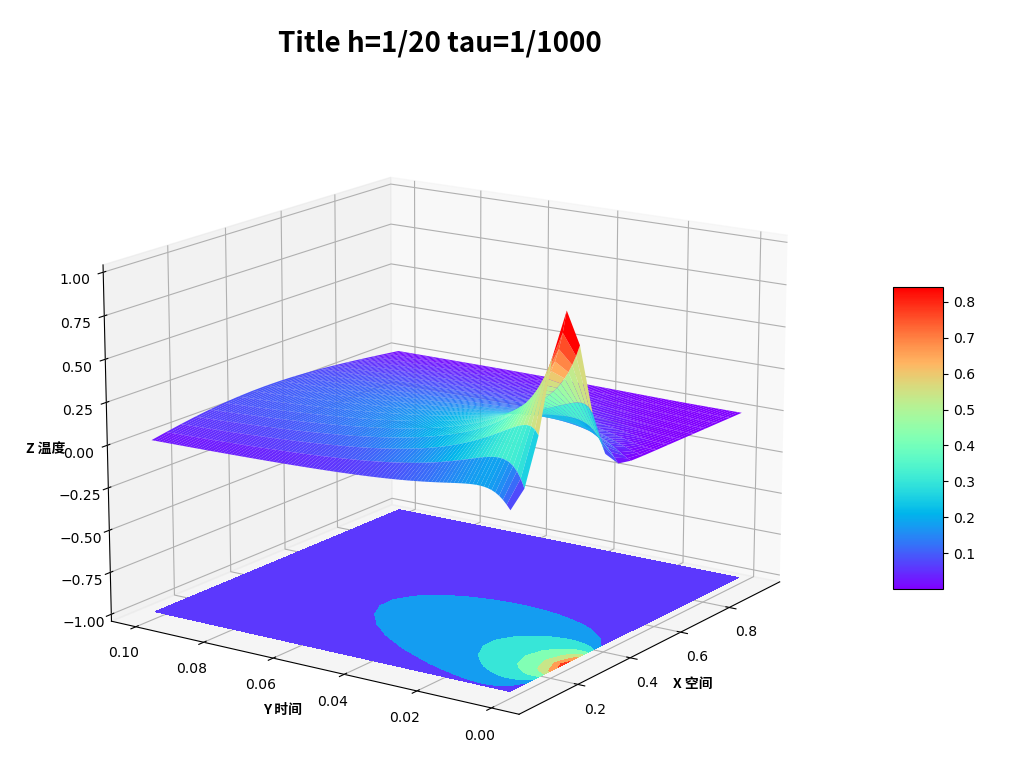
\includegraphics[scale=0.25]{2.png}
\caption{第一张结果图}
\end{figure}

\end{frame}

\begin{frame}[c]\frametitle{求解结果}

\begin{figure}
\centering
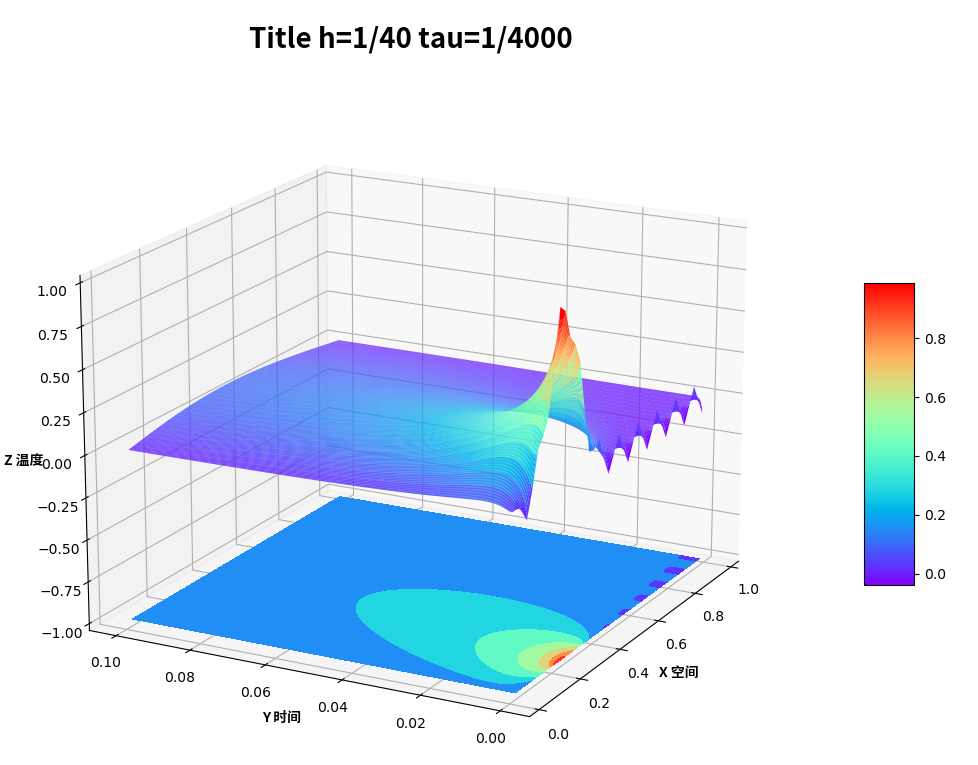
\includegraphics[scale=0.25]{3.png}
\caption{第二张结果图}
\end{figure}

\end{frame}

\begin{frame}[t]\frametitle{结果分析}

根据图一和图二可以看出,当随着空间划分更加的细,时间层数更多时,得到的结果几乎没有太大的变化,图二和图一不一样的地方只表现在迭代的初期,后期均趋于一致.还有就是此处的两张结果图中他们的时间步长是4倍关系,空间步长是2倍关系,这样的目的是因为向后差分格式的截断误差是$O(\tau + h^2)$,仅仅是为了分析截断误差的一种关系(前提是在已知真解的情况下,可以分析最大规模误差).

\end{frame}

\end{document}